%% Run LaTeX on this file several times to get Table of Contents,
%% cross-references, and citations.

\documentclass[11pt]{book}
\usepackage{Wiley-AuthoringTemplate}
\usepackage[sectionbib,authoryear]{natbib}% for name-date citation comment the below line
%\usepackage[sectionbib,numbers]{natbib}% for numbered citation comment the above line
\usepackage{array}
\usepackage{booktabs}
%%********************************************************************%%
%%       How many levels of section head would you like numbered?     %%
%% 0= no section numbers, 1= section, 2= subsection, 3= subsubsection %%
\setcounter{secnumdepth}{3}
%%********************************************************************%%
%%**********************************************************************%%
%%     How many levels of section head would you like to appear in the  %%
%%				Table of Contents?			%%
%% 0= chapter, 1= section, 2= subsection, 3= subsubsection titles.	%%
\setcounter{tocdepth}{2}
%%**********************************************************************%%

%\includeonly{ch01}
\makeindex
\usepackage{pdfpages}
\begin{document}
%Hello
\frontmatter
%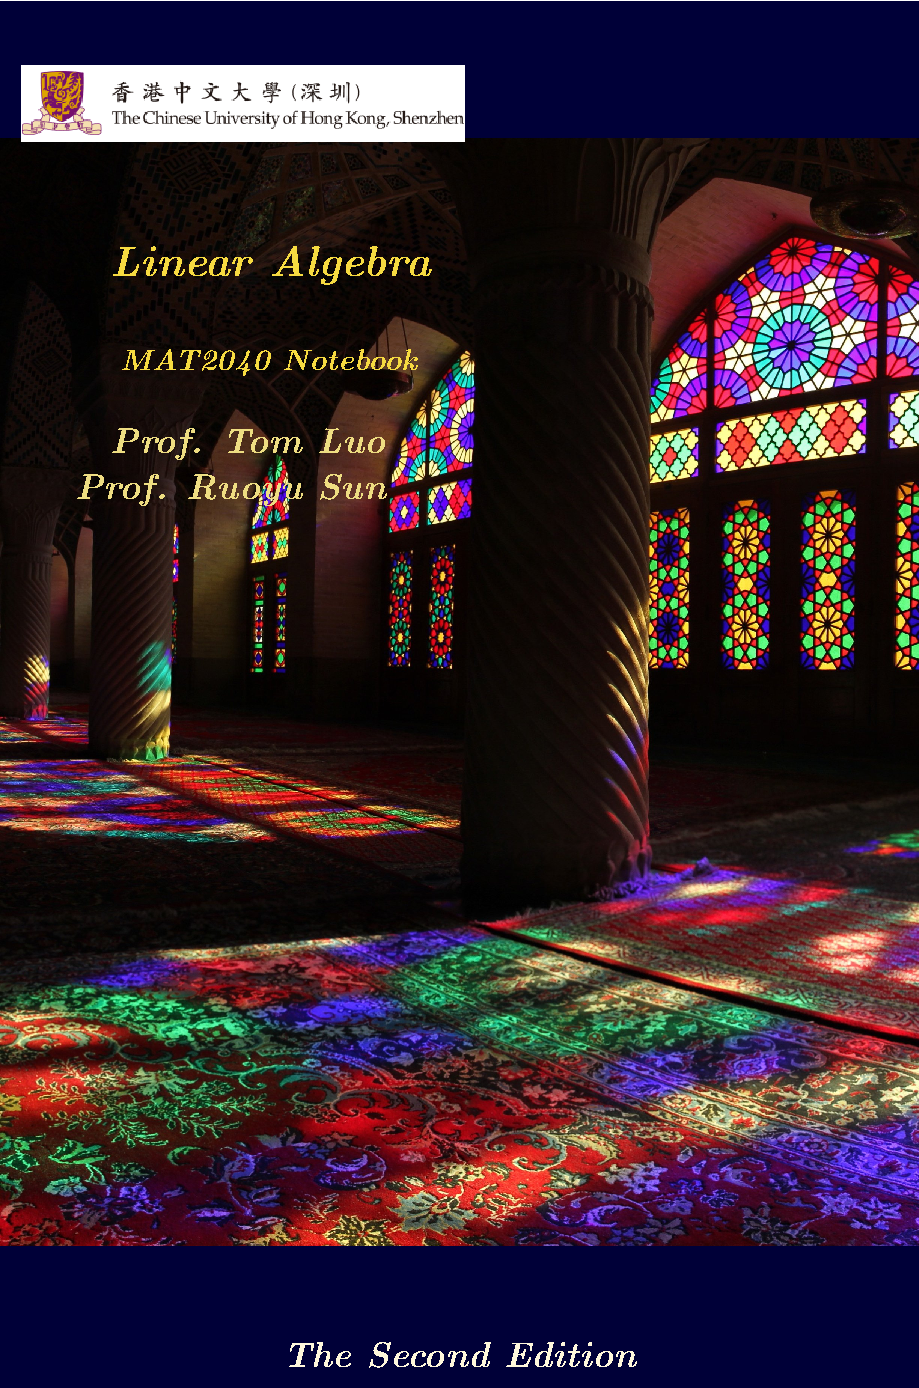
\includepdf[pages={1}]{book_cover/cover/FrontCover}
%%%%%%%%%%%%%%%%%%%%%%%%%%%%%%%%%%%%%%%%%%%%%%%%%%%%%%%%
%% Setting up title pages, type in the appropriate names here:

\booktitle{A Journey \\ In \\
Pure Mathematics}

\subtitle{MAT3006 $\&$ 3040 $\&$ 4002  Notebook}

\AuAff{Dr. Daniel Wong\\ The Chinese University of Hongkong, Shenzhen}
%\AuAff{Prof. Ruoyu Sun\\ University of Illinois Urbana-Champaign}
%% \\ will start a new line.


%% Print Half Title and Title Page:
\halftitlepage
\titlepage

%%%%%%%%%%%%%%%%%%%%%%%%%%%%%%%%%%%%%%%%%%%%%%%%%%%%%%%%
%% Copyright Page
%\begin{copyrightpage}{year}
%Title, etc
%\end{copyrightpage}

% Note, you must use \ to start indented lines, ie,
% 
% \begin{copyrightpage}{2004}
% Survey Methodology / Robert M. Groves . . . [et al.].
% \       p. cm.---(Wiley series in survey methodology)
% \    ``Wiley-Interscience."
% \    Includes bibliographical references and index.
% \    ISBN 0-471-48348-6 (pbk.)
% \    1. Surveys---Methodology.  2. Social 
% \  sciences---Research---Statistical methods.  I. Groves, Robert M.  II. %
% Series.\\
%
% HA31.2.S873 2004
% 001.4'33---dc22                                             2004044064
% \end{copyrightpage}

%%%%%%%%%%%%%%%%%%%%%%%%%%%%%%%%%%%%%%%%%%%%%%%%%%%%%%%%
%% Only Dedication (optional) 
%\dedication{To my girlfriend Jianyu Yang}

\tableofcontents

%\listoffigures %optional
%\listoftables  %optional



% If your book has chapters written by different authors,
% you'll need a Contributors page.

% Use \begin{contributors}...\end{contributors} and
% then enter each author with the \name{} command, followed
% by the affiliation information.

% \begin{contributors}
% \name{Zhi-quan Luo,} Shenzhen Research Institute of Big Data, Lecturer
%
% \name{Ruoyu Sun,} Industrial and Enterprise Systems Engineering, Lecturer
%
% \name{Jie Wang,} The Chinese University of Hongkong, Shenzhen, Typer
% \end{contributors}

%%%%%%%%%%%%%%%%%%%%%%%%%%%%%%%%%%%%%%%%%%%%%%%%%%%%%%%%
% Optional Preface:
%\begin{preface}
%This book is intended for the foundation course MAT2040, which is the first course on the linear algebra. It aims to cover basic linear algebra knowledge and its simple applications. This book was first written in 2017, and it is reviewed and revised in 2018. We have corrected several mistakes shown in the previous book and modified some proofs a little bit to give readers better insights of linear algebra.  During the modification, we also refer to many reading materials, which are also recommended for you:
\begin{itemize}
\item
ENGG 5781 Course Notes by Prof. Wing-Kin (Ken) Ma,  CUHK, Hongkong, China,  http://www.ee.cuhk.edu.hk/$\sim$wkma/engg5781
\item
Roger A. Horn and Charles R. Johnson, Matrix Analysis (Second Edition), Cambridge University Press, 2012.
\item
S. Boyd and L. Vandenberghe, Introduction to Applied Linear Algebra (Vectors, Matrices, and Least Squares), Cambridge University Press, 2018.
\end{itemize}
The whole book can cover a semester course in a 14week, each section in which corresponds to a 2-hour lecture. If you read the whole book, and work some mini-exercises, you will learn a lot. We hope you will get the insights on linear algebra and apply them in your own subject.




%\prefaceauthor{}
%\where{CUHK(SZ)\\
% \today}
%\end{preface}
% ie,
% \begin{preface}
% This is an example preface.
% \prefaceauthor{R. K. Watts}
% \where{Durham, North Carolina\\
% September, 2004}

%%%%%%%%%%%%%%%%%%%%%%%%%%%%%%%%%%%%%%%%%%%%%%%%%%%%%%%%
% Optional Acknowledgments:

\acknowledgments
This book is from the MAT3006,MAT3040,MAT4002 in spring semester, 2018-2019.
\authorinitials{CUHK(SZ)}  


%%%%%%%%%%%%%%%%%%%%%%%%%%%%%%%%%%%%%%%%%%%%%%%%%%%%%%%%
% Optional notations:
\begin{notations}
\acro{$\mathbb{R}^n$}{$n$-dimensional real space}
\acro{$\mathbb{C}^n$}{$n$-dimensional complex space}
\acro{$\mathbb{R}^{m\times n}$}{set of all $m\times n$ real-valued matrices}
\acro{$\mathbb{C}^{m\times n}$}{set of all $m\times n$ complex-valued matrices}
\acro{$x_i$}{$i$th entry of column vector $\bm x$}
\acro{$a_{ij}$}{$(i,j)$th entry of matrix $\bm A$}
\acro{$\bm a_i$}{$i$th column of matrix $\bm A$}
\acro{$\bm a_i\trans$}{$i$th row of matrix $\bm A$}
\acro{$\mathbb{S}^n$}{set of all $n\times n$ real symmetric matrices, i.e., $\bm A\in\mathbb{R}^{n\times n}$ and $a_{ij}=a_{ji}$ for all $i,j$}
\acro{$\mathbb{H}^n$}{set of all $n\times n$ complex Hermitian matrices, i.e., $\bm A\in\mathbb{C}^{n\times n}$ and $\bar{a}_{ij}=a_{ji}$ for all $i,j$}
\acro{$\bm A\trans$}{transpose of $\bm A$, i.e, $\bm B=\bm A\trans$ means $b_{ji}=a_{ij}$ for all $i,j$}
\acro{$\bm A\Her$}{Hermitian transpose of $\bm A$, i.e, $\bm B=\bm A\Her$ means $b_{ji}=\bar{a}_{ij}$ for all $i,j$}
\acro{$\trace(\bm A)$}{sum of diagonal entries of square matrix $\bm A$}
\acro{$\bm 1$}{A vector with all $1$ entries}
\acro{$\bm 0$}{either a vector of all
zeros, or a matrix of all zeros}
\acro{$\bm e_i$}{a unit vector with the nonzero element at the $i$th entry}
\acro{$\mathcal{C}(\bm A)$}{the column space of $\bm A$}
\acro{$\mathcal{R}(\bm A)$}{the row space of $\bm A$}
\acro{$\mathcal{N}(\bm A)$}{the null space of $\bm A$}
\acro{$\Proj_{\mathcal{M}}(\bm A)$}{the projection of $\bm A$ onto the set $\mathcal{M}$}
\end{notations}
\mainmatter
\setcounter{page}{1}

%%%%%%%%%%%%%%%%%%%%%%%%%%%%%%%%%%%%%%%%%%%%%%%%%%%%%%%%
% Optional introduction:
%\begin{introduction}
%
%The word \textit {traffic} becomes \textit {teletraffic} in telecommunications, as communications becomes telecommunications to indicate technology use, e.g., conversation from some distance through phones or Internet. The term teletraffic covers all kinds of computer communication traffic and telecom traffic.  This book includes teletraffic loss models.
%\end{introduction}
\chapter{Week7}
\section{Monday for MAT3040}\index{Monday_lecture}
\paragraph{Reviewing}
Define the characteristic polynomial for an linear operator $T$:
\[
\mathcal{X}_T(x)= \det((T)_{\mathcal{A},\mathcal{A}} - x\bm I)
\]
We will use the notation ``$I/\bm I$'' in two different occasions:
\begin{enumerate}
\item
$I$ denotes the identity transformation from $V$ to $V$ with $I(\bm v)=\bm v,\forall\bm v\in V$
\item
$\bm I$ denotes the identity matrix $(I)_{\mathcal{A},\mathcal{A}}$, defined based on any basis $\mathcal{A}$.
\end{enumerate}

\subsection{Minimal Polynomial}
\begin{definition}[Linear Operator Induced From Polynomial]
Let $f(x):=a_mx^m+\cdots+a_0$ be a polynomial in $\mathbb{F}[x]$, and $T:V\to V$ be a linear operator.
Then the mapping
\[
f(T)=a_mT^m+\cdots+a_1T+a_0I:\quad
V\to V,
\]
is called a linear operator induced from the polynomial $f(x)$.
\end{definition}

\begin{definition}[Minimal Polynomial]
Let $T:V\to V$ be a linear operator.
The \emph{minimal polynomial} $m_T(x)$ is a \emph{nonzero monic polynomial} 
of least (minimal) degree such that 
\[
m_T(T)=\bm0_{V\to V}.
\]
where $\bm0_{V\to V}$ denotes the zero vector in $\text{Hom}(V,V)$.
\end{definition}

\begin{example}
\begin{enumerate}
\item
Let $\bm A=\begin{pmatrix}
1&0\\0&1
\end{pmatrix}$, then $\bm A$ defines a linear operator:
\[
\begin{array}{ll}
A:&\mathbb{F}^2\to\mathbb{F}^2\\
\text{with}&\bm x\mapsto\bm A\bm x
\end{array}
\]
Here $\mathcal{X}_{ A}(x) = (x-1)^2$ and $\bm A-\bm I=\bm0$, which gives $m_A(x)=x-1$.
\item
Let $\bm B=\begin{pmatrix}
1&1\\0&1
\end{pmatrix}$, which implies
\[
\mathcal{X}_{ B}(x)=(x-1)^2,
\]
The question is that can we get the minimal polynomial with degree 1?

The answer is no, since $\bm B-k\bm I=\begin{pmatrix}
1-k&1\\0&1-k
\end{pmatrix}\ne\bm0$.

In fact, $m_B(x) = (x-1)^2$, since
\[
(\bm B-\bm I)^2=\begin{pmatrix}
0&1\\0&0
\end{pmatrix}^2=\begin{pmatrix}
0&0\\0&0
\end{pmatrix}.
\]
\end{enumerate}
\end{example}
%
%\begin{proposition}
%If $\bm A$ and $\bm B$ are similar, then
%\[
%m_{\bm A}(x)=m_{\bm B}(x).
%\]
%\end{proposition}
%\begin{proof}
%Left as exercise.
%\end{proof}
Two questions naturally arises:
\begin{enumerate}
\item
Does $m_T(x)$ exist? If exists, is it unique?
\item
What's the relationship between  $m_T(x)$ and $\mathcal{X}_T(x)$?
\end{enumerate}
Regarding to the first question, the minimal polynomial $m_T(x)$ may not exist, if $V$ has infinite dimension:
\begin{example}
Consider $V=\mathbb{R}[x]$ and the mapping
\[
\begin{array}{ll}
T:&V\to V\\
&p(x)\mapsto\int_0^xp(t)\diff t
\end{array}
\]
In particular, $T(x^n)=\frac{1}{n+1}x^{n+1}$.
Suppose $m_T(x)$ is with degree $n$, i.e., 
\[
m_T(x) = x^n +\cdots+a_1x+a_0,
\]
then 
\[
m_T(T)=T^n+\cdots+a_0I\ \text{is a zero linear transformation}
\]
It follows that
\[
[m_T(T)](x) = \frac{1}{n!}x^n+a_{n-1}\frac{1}{(n-1)!}x^{n-1}+\cdots+a_1x+a_0=0_{\mathbb{F}},
\]
which is a contradiction since
the coefficients of $x^k$ is nonzero on LHS for $k=1,\dots,n$, but zero on the RHS.
\end{example}

\begin{proposition}\label{pro:7:1}
The minimal polynomial $m_T(x)$ always exists for $\dim(V)=n<\infty$.
\end{proposition}
\begin{proof}
It's clear that $\{I,T,\dots,T^n,T^{n+1},\cdots,T^{n^2}\}\subseteq\text{Hom}(V,V).$
Since $\dim(\text{Hom}(V,V))=n^2$, we imply $\{I,T,\dots,T^n,T^{n+1},\cdots,T^{n^2}\}$ is linearly dependent, i.e., there exists $a_i$'s that are not all zero such that
\[
a_0I+a_1T+\cdots+a_{n^2}T^{n^2}=0
\]
i.e., there is a polynomial $g(x)$ of degree less than $n^2$ such that $g(T)=0$.

The proof is complete.
\end{proof}
%\paragraph{Assumption}
%We will asssume $V$ has finite dimension from now on.

\begin{proposition}\label{pro:7:2}
The minimal polynomial $m_T(x)$, if exists, then it exists uniquely.
\end{proposition}
\begin{proof}
Suppose $f_1,f_2$ are two distinct minimal polynomials with $\text{deg}(f_1)=\text{deg}(f_2)$.
It follows that
\begin{itemize}
\item
$\text{deg}(f_1-f_2)<\text{deg}(f_1)$.
\item
$f_1-f_2\ne0$
\item
$(f_1-f_2)(T) = f_1(T) - f_2(T)=0_{V\to V}$
\end{itemize}
By scaling $f_1-f_2$, there is a monic polynomial $g$ with lower degree satisfying $g(T)=0,$
which contradicts the definition for minimal polynomial.
\end{proof}

\begin{proposition}\label{pro:7:3}
Suppose $f(x)\in\mathbb{F}[x]$ satisfying $f(T)=\bm0$, then
\[
m_T(x)\mid f(x).
\]
\end{proposition}
\begin{proof}
It's clear that $\text{deg}(f)\ge\text{deg}(m_T)$.
The division algorithm gives 
\[
f(x)=q(x)m_T(x)+r(x).
\]
Therefore, for any $\bm v\in V$
\[
[r(T)](\bm v) = [f(T)](\bm v) - [q(T)m_T(T)](\bm v)=\bm0_V-q(T)\bm0_{V}=\bm0_V-\bm0_V=\bm0_{V}
\]
Therefore, $r(T) = \bm0_{V\to V}$.
By definition of minimal polynomial, we imply $r(x)\equiv0$.
\end{proof}
\begin{proposition}\label{pro:7:4}
If $\bm A,\bm B\in\mathbb{F}^{n\times n}$ are similar to each other, then $m_A(x) = m_B(x)$.
\end{proposition}
\begin{proof}
Suppose that $\bm B= \bm P^{-1}\bm A\bm P$, and that 
\[
\begin{array}{ll}
m_A(x)=x^k+\cdots+a_1x+a_0,
&
m_B(x)=x^{\ell}+\cdots+b_0.
\end{array}
\]
It follows that
\begin{align*}
m_A(\bm B)&=\bm B^k+\cdots+a_0I\\
&=\bm P^{-1}\bm A^k\bm P+\cdots+a_0\bm P^{-1}\bm P\\
&=\bm P^{-1}(\bm A^k+\cdots+a_0\bm I)\bm P\\
&=\bm P^{-1}(m_{A}(\bm A))\bm P
\end{align*}
Therefore, $m_A(\bm B)=\bm0$ since $m_{A}(\bm A)=\bm0$. By proposition~(\ref{pro:7:3}), we imply $m_{B}(x)\mid m_{A}(x)$. 
Similarly, $m_A(x)\mid m_B(x)$. 
Since $m_A(x)$ and $m_B(x)$ are monic, we imply $m_A(x)=m_B(x)$.
\end{proof}
\begin{remark}
Proposition~(\ref{pro:7:4}) claims that the minimal polynomial is \emph{similarity-invariant}; actually, the characteristic polynomial is \emph{similarity-invariant} as well.
\end{remark}
\paragraph{Assumption}
We will asssume $V$ has finite dimension from now on.
Now we study the vanishing of a single vector $\bm v\in V$.
\paragraph{Notation}
The $m_T(x)$ is a nonzero monic poylnomial of least degree such that 
\[
m_T(T)=\bm0_{V\to V}.
\]
\subsection{Minimal Polynomial of a vector}

\begin{definition}[Minimal Polynomial of a vector]
Similar to the minimal polynomial, we define the \emph{minimal polynomial of a vector $\bm v$ relative to $T$}, say $m_{T,\bm v}(x)$, as the monic polynomial of least degree such that 
\[
m_{T,\bm v}(T)(\bm v)=0
\]
\end{definition}
The existence of minimal polynomial of a vector is due to the existence of minimal polynomial; the uniqueness follows similarly as in proposition~(\ref{pro:7:2}).

\begin{proposition}
Let $T:V\to V$ be a linear operator and $\bm v\in V$.
The degree of the minimal polynomial of a vector is upper bounded by:
\[
\text{deg}(m_{T,\bm v}(x))\le \dim (V).
\]
\end{proposition}
\begin{proof}
It's clear that $\{\bm v,T\bm v,\dots,T^n\bm v\}\subseteq V$ and the proof follows similarly as in proposition~(\ref{pro:7:1}).
\end{proof}

Similar to the division property in proposition~(\ref{pro:7:3}), we have the division proprty for minimal polynomial of a vector:
\begin{proposition}\label{pro:7:6}
Suppose $f(x)\in\mathbb{F}[x]$ satisfying $f(T)(\bm v)=\bm0_{V}$, then
\[
m_{T,\bm v}(x)\mid f(x).
\]
In particular, $m_{T,\bm v}\mid m_T(x)$.
\end{proposition}

\begin{proof}
The proof follows similarly as in proposition~(\ref{pro:7:3}).
\end{proof}

\begin{proposition}
Suppose that $m_{T,\bm v}(x)= f_1(x)f_2(x)$, where $f_1,f_2$ are both monic. Let $\bm w = f_1(T)\bm v$, then
\[
m_{T,\bm w}(x) = f_2(x)
\]
\end{proposition}
\begin{proof}
\begin{enumerate}
\item
\[
f_2(T)\bm w = f_2(T)f_1(T)\bm v = m_{T,\bm v}(T)\bm v=\bm0
\]
By the proposition~(\ref{pro:7:3}), we imply 
$
m_{T,\bm w}|f_2
$.
\item
On the other hand,
\[
\bm0 = m_{T,\bm w}(T)(\bm w) = m_{T,\bm w}(T)f_1(T)\bm v= f_1(T)m_{T,\bm w}(T)\bm v,
\]
which implies that $m_{T,\bm v}(x)\mid f_1(x)m_{T,\bm w}(x),$, i.e.,
\[
f_1\cdot f_2\mid f_1\cdot m_{T,\bm w}\implies
f_2\mid m_{T,\bm w}.
\]
The proof is complete.
\end{enumerate}
\end{proof}


















\backmatter
%\appendix
\chapter{This is Appendix Title}

\section{This is First Level Heading}
\lipsum[1-2]

\subsection{This is Second Level Heading}
\lipsum[3]

\subsubsection{This is Third Level Heading}
\lipsum[4]

\paragraph{This is Fourth Level Heading}
\lipsum[5]

\subparagraph{This is Fifth Level Heading}
\lipsum[6]
\begin{theorem}
asfasf
\end{theorem}
\begin{theorem}
asfasf
\end{theorem}
%\backmatter

%\bibliography{wiley}%


%
\includegraphics{AuthorIcon}

\latexprintindex

\end{document} 
